\section{Алгоритм топологической сортировки. Применить алгоритм топологической сортировки.}

Если для двух вершин $v$ и $u$ есть маршрут из $v$ в $u$, но нет маршрута из $u$ в $v$,
то говорят, что $v$ предшествует $u$, а $u$ - последующее для $v$.

Алгоритм располагает вершины в последовательность таким образом, чтобы
если в построенной последовательности вершина $v$ находится правее
вершины $u$, то $u$ - последующее для $v$ в исходном графе или же $v$ и $u$ не
сравнимы в исходном бинарном отношении.

При работе алгоритма могут получитлься различнык последовательности.

Алгоритм работает на графах, в которых нет циклов,
содержащих более одного ребра. (то есть в графе могут быть циклы вида $vev$,
это значит, что вершина может иметь петлю).

Алгоритмы, которые рассмотрены ниже, работают на
ациклических графах. Если же в графах есть петли, а при удалении петель они
становятся ациклическими, то предварительно перед применением алгоритма
их нужно удалить.

Алгоритм топологической сортировки:
\begin{enumerate}[left=0.0em, labelsep=1em, topsep=0.0em, itemsep=0pt, parsep=0.5em]
    \item $i=1$
    \item В графе находим вершину, в которую не заходит ни одно ребро.
    Присваиваем ей номер $i$. Удаляем эту вершину и инцидентные ей рёбра.
    \item $i=i+1$
    \item Переходим к шагу 2 до тех пор, пока не пронумеруем все вершины.
\end{enumerate}

Выше графический способ

\newpage
\textbf{Алгоритм Кана (формализация графического метода)}

Пусть дан ациклический ориентированный простой граф . Для каждой
вершины графа $v$ находим $A(v)$ - множество таких вершин $u$ графа, что в
графе есть ребро $(u,v)$. То есть $A(v)$ — множество всех вершин, из которых
есть ребро в вершину $v$.

\begin{enumerate}[left=0.0em, labelsep=1em, topsep=0.0em, itemsep=0pt, parsep=0.5em]
    \item Для всех вершин находим $A(v)$
    \item $i=1$
    \item В графе находим вершину, для которой $A(v) = \varnothing$. Присваиваем этой
    вершине номер $i$. Удаляем эту вершину из всех множеств $A(v)$.
    \item $i=i+1$
    \item Переходим к шагу 3 до тех пор, пока не пронумеруем все вершины.
\end{enumerate}

\textbf{Опишем матричный способ:}

\begin{enumerate}[left=0.0em, labelsep=1em, topsep=0.0em, itemsep=0pt, parsep=0.5em]
    \item Рассмотрим матрицу смежности $A$ графа. Найдём в этой матрице
    нулевые столбцы. Вершины, соответствующие этим столбцам, нумеруем.
    Вычёркиваем столбцы и строки, соответствующие этим вершинам.
    \item Переходим к шагу 1 до тех пор, пока не пронумеруем все вершины.
\end{enumerate}

Пример:
\begin{figure}[h]
    \centering
    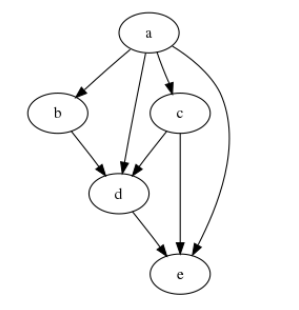
\includegraphics[scale=0.5]{12.png}
\end{figure}

\newpage
Применим алгоритм Кана к графу:
\begin{table}[h!]
    \centering
    \begin{tabular}{|c|c|c|c|c|c|c|c|}
        \hline
        iter & $i$ & $A(a)$ & $A(b)$ & $A(c)$ & $A(d)$ & $A(e)$ & set \\
        \hline
        0 &  & $\varnothing$ & $\{a\}$ & $\{a\}$ & $\{a,b,c\}$ & $\{a,c,d\}$ & $\varnothing$ \\
        \hline
        1 & 1 & $\varnothing$ & $\varnothing$ & $\varnothing$ & $\{b,c\}$ & $\{c,d\}$ & $a$ \\
        \hline
        2 & 2 & $\varnothing$ & $\varnothing$ & $\varnothing$ & $\varnothing$ & $\{d\}$ & $a,b$ \\
        \hline
        3 & 3 & $\varnothing$ & $\varnothing$ & $\varnothing$ & $\varnothing$ & $\varnothing$ & $a,b,c$ \\
        \hline
        4 & 4 & $\varnothing$ & $\varnothing$ & $\varnothing$ & $\varnothing$ & $\varnothing$ & $a,b,c,d$ \\
        \hline
        5 & 5 & $\varnothing$ & $\varnothing$ & $\varnothing$ & $\varnothing$ & $\varnothing$ & $a,b,c,d,e$ \\
        \hline
    \end{tabular}
\end{table}

Результат работы алгоритма: $a, b, c, d, e$.

Пример:
\begin{figure}[h]
    \centering
    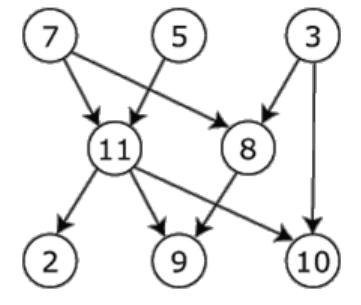
\includegraphics[scale=0.5]{12_2.png}
\end{figure}

Для графа существует несколько согласованных последовательностей его
вершин, которые могут быть получены при помощи топологической
сортировки, например: $7,5,3,11,8,2,9,10; 3,7,5,8,11,10,9,2$.

Видно, что в последовательности могут быть переставлены любые две
стоящие рядом вершины, которые не входят в отношение частичного
порядка (несравнимы)